\chapter{Ergebnis und Diskussion}
\label{ch:ergebnis}

Jeder der insgesamt 2400 Testdurchläufe benötigte im Mittel 34,2 CPU-Kern-Stunden bei CPUs mit durchschnittlich 2.4GHz, wobei der \acs{DDPGA} um 30\% schneller und der \acs{DDRQLA} vier Mal langsamer trainierte. Dies ergibt eine Gesamtlaufzeit auf einer CPU von etwas über $82.000$ Stunden.

In diesem Kapitel werden die Ergebnisse basierend auf dem experimentellen Aufbau aus Kapitel \ref{ch:evaluationsaufbau} vorgestellt.
Dies umfasst Einblicke in das Hyperparametertuning und Training (\ref{sec:reshyp}), die Ergebnisse der Vorstudie zur Eingrenzung der \acs{DRL} Varianten (\ref{sec:voragentenerg}), die Analyse verschiedener Architekturen im Hinblick auf unterschiedliche Wertpapiercluster mit den Resultaten der Hauptevaluation (\ref{sec:erghaupteval}), die Ergebnisse des dritten Experiments für eine Einschätzung der Agenten in Krisenzeiten (\ref{sec:covid}), und die Performanceanalyse des vierten Experiments zur Evaluation, inwieweit einzelne Erweiterungen in der Architektur Einfluss auf \acs{DRL} Strategien nehmen (\ref{sec:erweiterteragent}).
Welchs t-test mit einem Signifikanzniveau von $p=0,05$ wurde verwendet, um die Zusammenhänge einiger Charakteristika und Hyperparameter zu untersuchen.

\section{Training und der Einfluss von Hyperparametern}
\label{sec:reshyp}

Für alle Experimente können auffällig hohe Schwankungen in der Trainingsdauer verschiedener Durchläufe desselben Agenten wegen early stopping beobachtet werden. 
Teilweise bricht der Algorithmus nach weniger als 30 Iterationen ab, während er bei gleicher Hyperparameterkombination auf demselben Wertpapier mehr als 800 Trainingsdurchläufe iteriert.
Die Endresultate der Trainingsiterationen oszillieren meistens, wodurch der Eindruck entsteht, dass der Lernalgorithmus häufig keinen stetigen Fortschritt macht.
Hohe Schwankungen sind ebenfalls bei der Bestimmung der optimalen Hyperparameter für jede Kombination aus Wertpapier und Agent zu beobachten,
was vermutlich auf unterschiedliche Marktmuster 2018 und 2019 zurückzuführen ist.
Die Parameter weisen auch bei Vergleichen von Branchen oder Wertpapierklassen keine statistisch signifikanten Tendenzen auf, welche Einstellungen optimal sind. Nichtsdestotrotz kann durch einen Vergleich der durchschnittlichen Ergebnisse der Validation mit den Testresultaten der klare Trend beobachtet werden, dass Modelle mit einer Hyperparameteroptimierung besser abschneiden.
Das bestätigt, dass die Konfiguration der Modelle trotz Marktfluktuationen ein essentieller Schritt für das Training von \acs{DRL} Algorithmen im algorithmischen Handel ist. 

\paragraph{Detaillierte Analyse.}
Genauere Untersuchungen zeigen jedoch, dass bei einer guten Performance einer Hyperparameterkombination im Validationsatz nicht eindeutig auch gute Ergebnisse im Testsatz zu erwarten sind.
Obwohl beispielsweise eine Verringerung von epsilon decay oder gamma zu höheren Profiten bei der Validation führt, konnten damit in allen drei Testjahren schlechtere Ergebnisse erzielt werden.
Genauso sorgt eine Änderung der Speicher- oder Schichtgröße auf dem Validationssatz beim zweiten Experiment nur für einen Performanceunterschied von unter einem Prozent.
Auf dem Testsatz hingegen führt eine größere verdeckte Schicht bzw. ein längerer Speicherhorizont zu hohen Verlusten in 2018, wenngleich damit 2019 und in Experiment 3 der dreifache Gewinn erzielt wird.
Statistisch korreliert eine höhere Schichtgröße signifikant positiv\footnote{Der gemittelte Anteil der gehaltenen Wertpapiere am Portfoliowert in Bezug auf jeden Agenten für jedes Wertpapier korreliert signifikant mit der Schichtgröße mit einem p-Wert von ca. $p=0,0477$.} mit der Zahl der gehaltenen Wertpapiere, was das Gefälle in den Experimenten erklären könnte. 
Weiterhin enthält die optimale Hyperparameterkombination im Jahr 2019 etwas über 28\% häufiger den geringeren Wert für die Schichtgröße. 
Dies ist darin begründet, dass weniger gehandeltene Wertpapiere zu weniger Verlust im Validationsjahr führen.

Die obigen Tendenzen lassen sich bis auf eine Ausnahme auf jeden Agenten individuell übertragen. Und zwar verzeichnet der \acs{DQLA} bei einer Erhöhung von epsilon decay signifikant höhere Verluste, durchschnittlich ca. 35,7\%. Ein langsamerer Zerfall von epsilon nimmt demnach positiven Einfluss auf die Konvergenz im Training und die Performance im Test.
Analog verbessert der \acs{DDPGAK} zusätzlich noch die Batchgröße und den Parameter $\tau$. 
Wie erwartet ist die Batchgröße ein wichtiger Hyperparameter, der die Performance des \acs{DDPG} Netzwerks beeinflusst. Der Agent trainiert bei einer höheren Batchgröße schneller, jedoch mit einer höheren Varianz in den Renditen.
Der Parameter $\tau$ hingegen beeinflusst weder die Ergebnisse der Validation noch der Tests in signifikantem Maße, da bei einer Änderung von $\tau$ für keinen Agenten in keinem der Jahre eine klare Tendenz erkennbar ist.

\section{Vorauswahl der Agenten}
\label{sec:voragentenerg}

Die Ergebnisse der Voranalyse decken sich in größten Teilen mit der bestehenden Literatur (cf. Tabelle \hyperref[tabe1]{A1}). Vier verschiedene \acs{DQL} Agenten konnten sich gegenüber anderen \acs{DRL} Ansätzen wie in \parencite{duel,deepQtrader,zhang2019deep} durchsetzen. Dueling Strategien bzw. andere Abwandlungen des \acs{DQL} Algorithmus (vgl. Double \acs{DQL} in \parencite{zhang2019deep}) zeigen analog zu \parencite{zhang2019deep} keine bessere Vorhersagekraft. Darüber hinaus verbessern rekurrente Architekturen die Performance im Durchschnitt (vgl. \parencites{recubetter}) um mehr als 12\%, was später in der Hauptevaluation noch deutlicher wird.
Ein unerwartetes Ergebnis der initialen Studie ist, dass der einfache \acs{DQLA} und \acs{DDPGA} zu besseren Resultaten als dessen rekurrente Variante führen. Überdies schneidet die Kombination aus der Dueling Architektur (\acs{DDQL}) mit einer \acs{LSTM} Schicht entgegen der zuvor beschriebenen Erwartung unter allen Varianten am besten ab.

\section{Hauptevaluation}
\label{sec:erghaupteval}

Da die Agenten auf verschiedenen Wertpapierclustern unterschiedliche Resultate liefern, werden Performanceunterschiede in Bezug auf die charakteristischen Merkmale aus Abschnitt \ref{sec:datensatz} und deren Wechselwirkungen sowohl durchschnittlich als auch individuell für jede Variante analysiert.
Es gilt zu beachten, dass die Ergebnisse in Abbildung \ref{fig:boxplot} stark von der verwendeten Testumgebung beeinflusst sind; jede Schlussfolgerung daraus beschränkt sich folglich spezifisch auf das gewählte Setting und den Zeithorizont.

\begin{figure}[t!]
\center
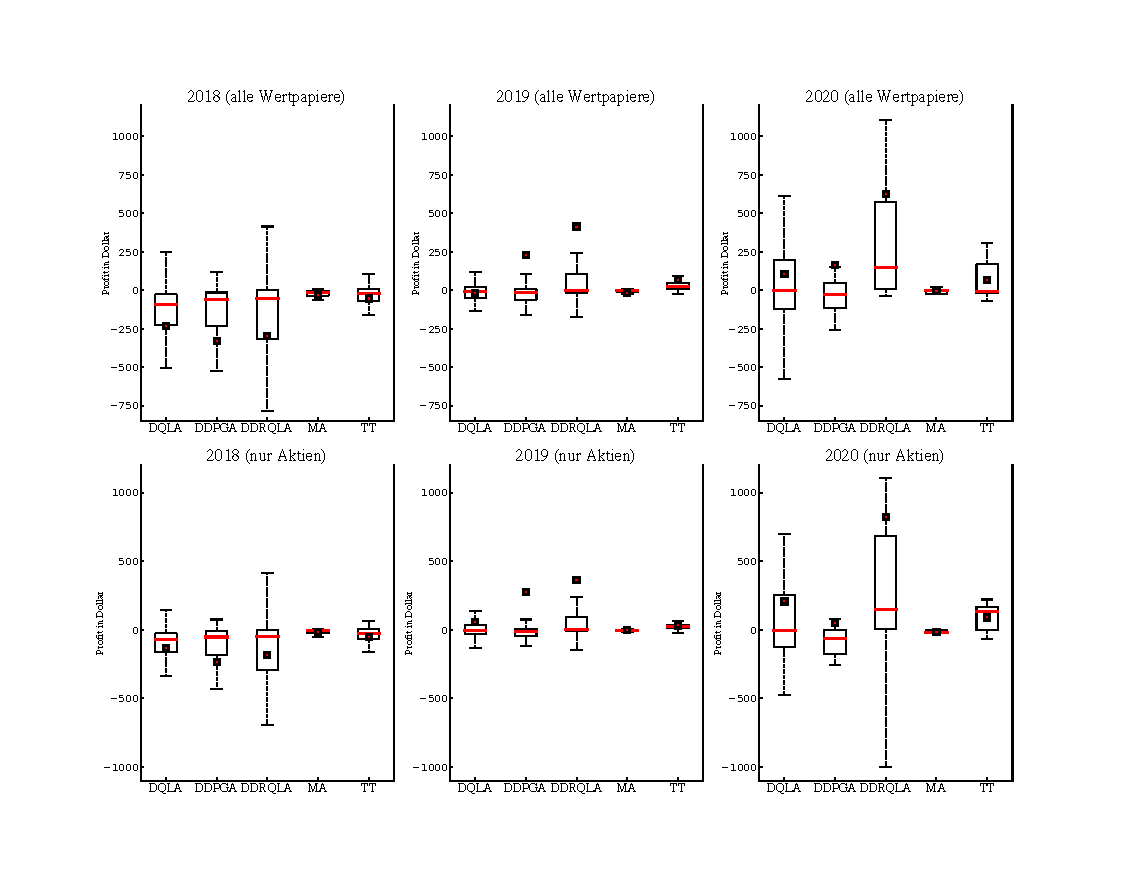
\includegraphics[scale=0.95]{figures/plot.pdf}
\vspace{0.1mm}
\caption[Ergebnisse der \acs{DRL} Agenten ohne Kontextdaten]{Ergebnisse aller 1440 Testdurchläufe der \acs{DRL} Agenten ohne Kontextdaten für alle Wertpapiere (oben) und nur für Aktien (unten) für jede Variante und jedes Evaluationsjahr. Die Kästen repräsentieren die Reichweite zwischen dem 25ten und 75ten Perzentil der Werte, während die Pfeile bis auf Ausreißer die gesamte Reichweite illustrieren. Der rote Punkt zeigt den Mittelwert und die rote Linie markiert den Median der Daten. Der Mittelwert weicht im zweiten Testjahr aufgrund hoher Ausreißer nach oben stark vom Median ab.}
  \label{fig:boxplot}
\end{figure}

Abbildung \ref{fig:boxplot} veranschaulicht die Verteilung der durchschnittlichen Ergebnisse jedes Agenten ohne Kontextdaten in Bezug auf deren Testjahr.
Agentenübergreifend ist zu sehen, dass durchschnittlich deutlich bessere Ergebnisse 2019 (145 \$) als 2018 (-185 \$) erreicht werden konnten.
Dieser Unterschied kann auf den längeren Trainingszeitraum und auf günstigere Marktbedingungen zurückgeführt werden.
Eine erste wichtige Erkenntnis daraus ist, dass durch eine gute Wahl des Testjahres die Agenten prozentual wesentlich weniger Verlust erleiden (42,0\%) als zuvor (65,3\%). Da selbst dieselben Agenten in unterschiedlichen Jahren hohe Varianzen in den Ergebnissen aufweisen, sind Performancevergleiche mit anderen Studien nur bei ähnlichem Setup sinnvoll.

Im Vergleich zu anderen Evaluationen mit kongruentem Testsetting schneiden die \acs{DRL} Varianten in den meisten Fällen leicht schlechter ab.
Für das Jahr 2018 liegt das beste Testergebnis auf einer Technologieaktie bei ungefähr 9\% Portfoliosteigerung, was weit unter den ca. 17\% von Théate et al. \parencite{théate2020application} liegt, die allerdings einen viel aufwendigeren Agenten und geringere Transaktionskosten verwenden.
Das beste Ergebnis im Jahr 2019 erzielte wie zu erwarten der \acs{DDRQLA} mit einem Gewinn von über 12\%, was auf der anderen Seite relativ nahe an die präsentierten Ergebnisse von \parencite{zhang2019deep,duel} herankommt.
Es gilt aber zu beachten, dass nicht state-of-the-art Ergebnisse erzielt werden sollen, sondern schwerpunktmäßig faire Vergleiche einzelner Varianten und Wertpapiercluster gemacht werden.

\paragraph{Vergleich der Agenten.}
Die großen Performanceunterschiede einzelner Varianten im oberen Teil von Abbildung \ref{fig:boxplot} zeigen, dass in der differenzierten Evaluation keine Architektur eindeutig bessere Ergebnisse liefert.
Während 2019 eine überlegene durchschnittliche Performance des \acs{DDRQLA} vor anderen \acs{DRL} Architekturen und den beiden Baseline Agenten beobachtet werden kann, schneidet er 2018 deutlich schlechter ab.
Trotz der hohen Varianz der Testergebnisse ist allerdings der Mittelwert des Sharpe Ratios der rekurrenten Variante in beiden Jahren am besten.
Dahinter weisen \acs{DDPG} Modelle durchschnittlich die besten Resultate auf, obwohl 2018 der \acs{DQLA} leicht dominiert. Dessen bessere Ergebnisse sind auf eine geringere Standardabweichung des Portfoliowertes zurückzuführen. Dies weist auf eine niedrigere Handelsfrequenz hin, was insbesondere geringere Verluste in moderaten Abschwungphasen wie in 2018 impliziert.

\paragraph{Vergleich der Charakteristika.}
Eine unerwartete Beobachtung dieser Studie ist, dass mit Aktien höhere Gewinne erzielt werden als mit Warentermingeschäften oder ETFs (siehe den unteren Teil von Abbildung \ref{fig:boxplot}).
In einer näheren Betrachtung werden Charakteristika in der Zeitreihe untersucht, mit denen die besseren Ergebnisse begründet werden können. 
Es zeigt sich, dass sowohl das Sharpe Ratio als auch die Performance signifikant\footnote{Konkret wird getestet, ob der gemittelte Profit für jede Komposition aus Agent und Wertpapier signifikant mit der Volatilität zusammenhängt.
Der Korrelationskoeffizient beträgt ca. -0,33.}
negativ mit der Volatilität einer Anlage korrelieren.
Dadurch dass Aktien mit 0,68 die geringste Standardabweichung gegenüber Waren (4,85) und ETFs (0,72) aufweisen, sind diese Anlagen in diesem Evaluationssetting vorteilhaft.
Genauer profitieren der \acs{DQLA} und der \acs{DDPGA} am meisten von der geringeren Volatilität, wohingegen der \acs{DDRQLA} 2019 sogar schlechter abschneidet.
Die Fähigkeit, besser auf alte Informationen durch die \acs{LSTM} Architektur zuzugreifen, scheint ausschlaggebend für eine gute Performance bei instabilen Wertentwicklungen zu sein.
Indes unterliegen stabile Wertpapiere weniger Spekulationen und Irregularitäten, womit die insgesamt bessere Mustererkennung erklären könnte.
Nicht signifikant ins Gewicht fällt hingegen der Kursverlauf eines Wertpapiers. 
Erwartungsgemäß beeinflusst ein wachsender Kursverlauf die Performance leicht positiv, ist aber zumindest in diesem Kontext nicht hinreichend für bessere Ergebnisse und zeigt ferner keinen signifikanten Zusammenhang mit der Performance.

Diese Schlussfolgerungen gelten für alle Charakteristika bis auf den Vergleich einzelner Branchen. 
In diesem Fall schneiden die Agenten 2019 bei Aktien von Unternehmen aus dem Gesundheitswesen trotz einer geringeren Volatilität und einer höheren Wertsteigerung schlechter ab.
Um diesen Zusammenhang zu untersuchen, wird der Einfluss des Beta-Faktors auf die Portfolioentwicklung für den Branchenvergleich zusätzlich untersucht.
Da Aktien aus dem Gesundheits- oder Finanzwesen einen niedrigen Beta-Faktor besitzen, korrelieren sie weniger stark mit dem Markt als Technologieaktien.
Diese Eigenschaft ist bei Aufwärtstrends wie beispielsweise im Jahr 2019 vorteilhaft, wenngleich Verluste in Abwärtstrends dadurch verstärkt werden.
Allgemein lässt sich in den Ergebnissen eine statistisch signifikante Abhängigkeit zwischen der Varianz des Portfolios und dem Beta-Faktor messen.
Demnach sollten Wertpapiere mit einem hohen Beta-Faktor nur bei einer risikofreudigen Nutzenfunktion eingesetzt werden. Für ein maximales Sharpe Ratio sollten jedoch Aktien gemieden werden, die sowohl eine hohe Volatilität als auch einen hohen Beta-Faktor besitzen. 

\section{Anwendung während der COVID-19 Pandemie}
\label{sec:covid}

Die rechten Schaubilder in Abbildung \ref{fig:boxplot} zeigen die überraschend gute Performance in Krisenzeiten.
Jede \acs{DRL} Variante erzielt in fast allen Fällen bessere Ergebnisse als die Baseline Agenten und weist sogar einen deutlich erhöhten Profit im Vergleich zum ersten Evaluationsjahr auf.
Nur die \acs{DDPG} Agenten weisen leicht schlechtere Tendenzen bei Aktien auf, speziell der \acs{DDPGAK} reduziert seine Handelsfrequenz auffällig drastisch. Eine mögliche Erklärung dafür ist der stark erhöhte \acs{^VIX}, der in den Trainingsjahren häufig positiv mit Verlusten korreliert.

\begin{figure}[t!]
\center
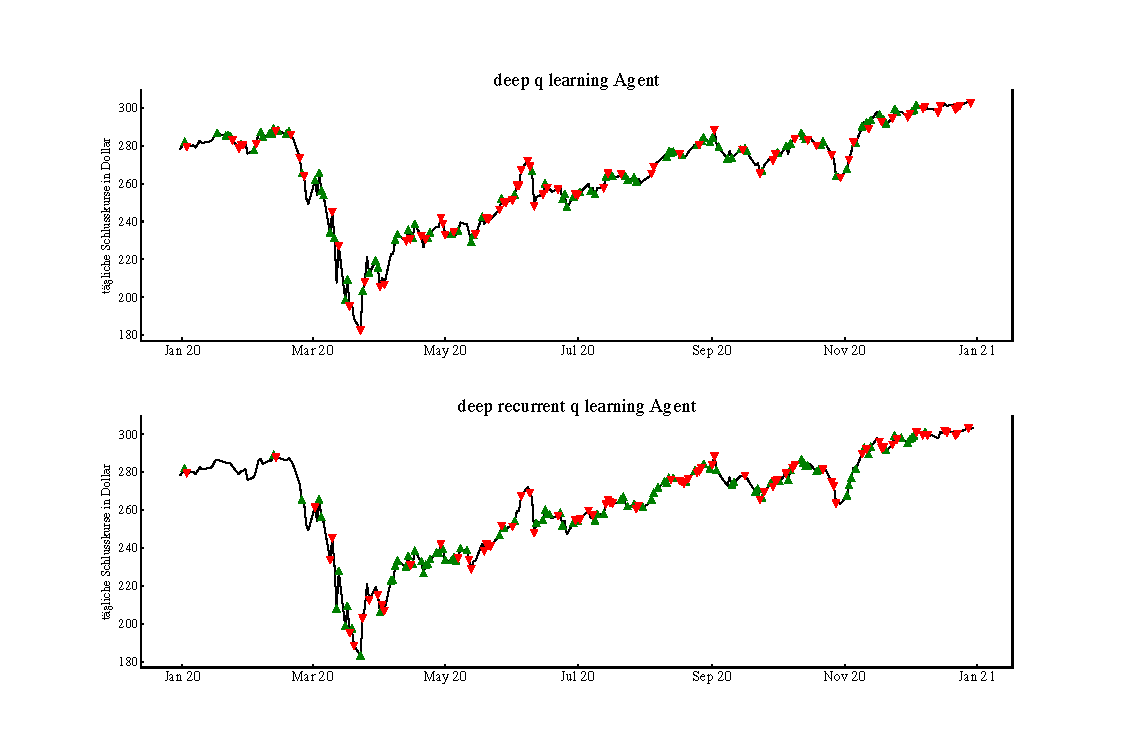
\includegraphics[scale=0.95]{figures/plot2.pdf}
\vspace{0.1mm}
\caption[Handlungsentscheidungen zweier Agenten während der COVID-19 Krise]{Ergebnisse des \acs{DQLA} (oben) und des \acs{DDRQLA} (unten). Die roten Pfeile signalisieren Verkaufszeitpunkte, grüne Pfeile zeigen Kaufzeitpunkte.}
  \label{fig:agentenspectime}
\end{figure}

Die beiden Schaubilder in Abbildung \ref{fig:agentenspectime} zeigen, wie sich die Handlungsentscheidungen des \acs{DDRQLA} und \acs{DQLA} der volatilen Krisenphase voneinander im Einzelnen unterscheiden:
Die Handlungen beider Agenten bleiben verzögert hinter dem Markttrend zurück. Jedoch reagiert der \acs{DDRQLA} besonders im ersten Quartal relativ früh auf die volatile Marktsituation, indem er seine Handelsfrequenz reduziert. Somit können hohe Verluste im späteren Verlauf vermieden werden.
Die deutlich bessere Rendite des \acs{DDRQLA} kann dadurch erklärt werden, dass anschließend im zweiten Quartal die günstige Marktsituation durch ein erhöhtes Kaufverhalten besser genutzt wird. 
Während der \acs{DQLA} sein tendenziell konservatives Kaufverhalten beibehält, profitiert der \acs{DDRQLA} von einer gierigen Strategie.
Diese Erkenntnis deckt sich mit den Schlussfolderung aus Abschnitt \ref{sec:erghaupteval}, dass die in Paragraph \ref{subsec:ddrqltheorie} beschriebenen Vorteile von \acs{LSTM} Schichten in volatilen Phasen deutlich die Performance verbessern.
Ferner kann der rekurrente Agent die Unterstützungszone\footnote{Eine Unterstützungszone ist ein Begriff in der technischen Analyse von Finanzdaten. Er beschreibt ein Niveau, bei dem ein sinkender Wertpapierkurs dazu tendiert, nach oben abzuprallen. Wird dieses Niveau durchbrochen, ist es wahrscheinlich, dass der Wertpapierkurs weiter fällt.} im vierten Quartal besser erkennen, aber aufgrund der Einschränkung des Aktionsraums nicht schnell genug seinen Bestand erhöhen.

Trotz einer erhöhten Volatilität sind die Agenten bei großen Marktveränderungen profitabel. 
Allerdings kann man wegen des eher kleinen Krisen-Datensatzes nicht gesichert von einer guten Performance in jeder Krisenzeit ausgehen. 
Da die Kurseinbrüche im ersten Quartal des Jahres eintreten, halten die Agenten aufgrund der strengen Handelsrestriktionen häufig nicht genügend Wertpapiere.
Für eine genauere Einschätzung muss in weiteren Studien der Testzeitraum der COVID-19 Pandemie variieren, damit die Auswirkungen des Kurseinbruchs in diversen Szenarien untersucht werden können.

\section{Einfluss der erweiterten Aspekte}
\label{sec:erweiterteragent}

Um detailliertere Erkenntnisse zu gewinnen, beschränkt sich die folgende Analyse auf Vergleiche zwischen Agenten, die denselben Trainingsalgorithmus verwenden.

\paragraph{Kontextdaten.}
Das Hinzufügen von Kontextdaten verbessert weder die Performance des \acs{DDPG} Algorithmus (\acs{DDPGAK}) noch des erweiterten \acs{DQL} Ansatzes (\acs{EDQLA}) in signifikantem Maße.
Obwohl für den \acs{DDPGAK} eine leicht bessere Performance in 2018 beobachtet wird, schneidet der Agent 2019 und 2020 schlechter ab.
Im Vergleich dazu erleidet der \acs{EDQLA} in den meisten Fällen durchschnittlich höhere Verluste, wobei allgemein ein instabileres Training mit einer signifikant längeren Laufzeit beobachtet werden kann.
Eine erhöhte Varianz sowohl bei der Validation als auch bei den Testergebnissen zeigt, dass die ergänzenden Marktinformationen in diesen simplen Modellen nicht vorteilhaft für die Entscheidungsfindung sind. 
Nichtsdestoweniger suggeriert eine qualitative Analyse der Handelszeitpunkte eine insgesamt geringfügig bessere Entscheidungsfindung in volatilen Phasen, die sich in einer reduzierten Handelsfrequenz bemerkbar macht.
Daraus lässt sich ableiten, dass Kontextdaten bei risikoreichen Konjunkturphasen unterstützend wirken können.
Da aber auch bei positivem Marktwachstum eine signifikant geringere Handelsfrequenz zu beobachten ist, können günstige Marktsituationen nur bedingt genutzt werden.

Wenngleich aufwendigere Agenten in einem anderen Setting \parencites{paperrepo2,startrader} mit Kontextdaten bessere Ergebnisse erzielen, 
können in dieser Evaluation durch korrelierende Marktinformationen keine signifikanten Unterschiede in der Performance beobachtet werden.
Gegeben, dass die zusätzlichen Finanzmarktdaten in großem Maße die Anzahl der Eingabewerte erhöhen, lohnt sich diese Modifikation aufgrund der höheren Komplexität unter den Limitationen von Kapitel \ref{ch:evaluationsaufbau} somit nicht.

\paragraph{Dropout.}

Änderungen in der Dropoutrate ändern nicht signifikant die Performance der modifizierten \acs{DQL} Variante, jedoch konnte das beste Ergebnis des Agenten in allen drei Jahren durch einen höheren Dropoutwert verbessert werden.
Da die Mittelwerte der Validations- und Testergebnisse weniger stark voneinander abweichen, lässt sich ein tendenziell weniger überangepasstes Modell beobachten.
Limitiert sind diese Schlussfolgerungen allerdings dadurch, dass der Effekt von Dropout nicht isoliert betrachtet werden kann.
Um genauere Aussagen über die Überanpassung des Modells zu treffen, müsste in einem gesonderten Experiment der \acs{DQLA} nur um die Regularisierungsmethode erweitert und den Einfluss auf die Performance statistisch analysiert werden. 
Das stellt ein interessantes zukünftiges Forschungsfeld dar, ist aber im Umfang dieser Bachelorarbeit nicht enthalten.

\paragraph{Aktionsraum.}

Die Erweiterung des Aktionsraums wirkt sich nicht signifikant auf die Performance des \acs{EDQLA} aus, aber führt besonders im Krisenjahr aufgrund eines deutlich erhöhten Wertpapierbestandes im ersten Quartal 2020 zu schlechteren Resultaten. 
Trotz schwächerer Handelseinschränkungen kann der \acs{DQL} Algorithmus ähnlich wie in Abbildung \ref{fig:agentenspectime} den Aufwärtstrend im zweiten Quartal nicht nutzen.
Stattdessen sorgt das erweiterte Framework dafür, dass wegen höherer Transaktionskosten volatile Phasen noch stärker die Performance beeinträchtigen.
Statistisch kann ein erhöhter Korrelationskoeffizient um $41\%$ für den negativen Zusammenhang der Volatilität mit der Performance nachgewiesen werden.

Allgemein investiert der Agent deutlich mehr, wodurch wie zu erwarten auch stärkere Ausreißer nach unten zu beobachten sind.
Der Agent kann demnach die in Abschnitt \ref{sec:erweiterung} beschriebene Handelseinschränkung überwinden und einen größeren Teil seines Bargeldes nutzen, besitzt aber dadurch höhere Varianzen in den Ergebnissen. 
Folglich besitzt der Agent ein durchschnittlich geringeres Sharpe Ratio als der einfachere \acs{DQLA}.
Eine wichtige Folgerung aus diesem Experiment ist daher, dass bei einem simplen \acs{DQL} Algorithmus mehr Handelsmöglichkeiten zu höherem Risiko führen.
Allerdings mindern Transaktionskosten hohe Gewinne, weshalb diese Erweiterung für das verwendete Modell nicht eingesetzt werden sollte.




